\documentclass[11pt,a4paper,english]{ceurart}

\sloppy

\usepackage{tikz}
\usetikzlibrary{shapes.geometric, arrows, positioning, fit, backgrounds}

\begin{document}

\copyrightyear{2026}
\copyrightclause{Copyright for this paper by its authors. Use permitted under Creative Commons License Attribution 4.0 International (CC BY 4.0).}
\conference{IberLEF 2026, September 2026, Le\'on, Spain}

\title{MBART-50 Based Transfer Learning for Bidirectional MSL-Spanish Translation}

\author[1]{Miguel Bethencourt Mayedo}[%
orcid=0000-0001-8873-6802,
email=bethencourt.may@gmail.com,
]
\cormark[1]
\address[1]{Universidad de Camag\"uey, 70100, Cuba}

\cortext[1]{Corresponding author.}

\begin{abstract}
This paper describes my submission to the MSLG-SPA 2026 shared task at IberLEF 2026, which focuses on bidirectional translation between Mexican Sign Language (MSL) glosses and Spanish. Due to the low-resource nature of the task (only 489 official training pairs), my approach leverages transfer learning utilizing the pre-trained multilingual sequence-to-sequence model mBART-50 Large. I implemented a four-phase training pipeline consisting of: (1) domain adaptation using the German PHOENIX-2014-T sign language dataset to establish a baseline understanding of spatial grammar; (2) large-scale synthetic data generation via rule-based back-translation of 10,000 Spanish sentences from the OPUS corpus into pseudo-glosses; (3) 5-fold cross-validation fine-tuning on the official competition dataset; and (4) inference employing optimized beam search decoding strategies. The final official evaluation yielded the following results: my system achieved a COMET score of 0.6813 and a BLEU score of 16.6254 in the MSLG-to-Spanish translation subtask (Subtask A), and a BLEU score of 11.7564 in the Spanish-to-MSLG translation subtask (Subtask B). These outcomes highlight both the potential of pre-trained models for sign language translation and the methodological limitations of my current approach. Specifically, my reliance on a standard full fine-tuning process resulted in suboptimal parameter adaptation. I analyze these limitations and propose the integration of Parameter-Efficient Fine-Tuning (PEFT) techniques, particularly Low-Rank Adaptation (LoRA), to mitigate overfitting risks and improve generalization in future low-resource sign language translation tasks.
\end{abstract}

\begin{keywords}
  Mexican Sign Language \sep
  Machine Translation \sep
  mBART-50 \sep
  Transfer Learning \sep
  Low-Resource NLP \sep
  Data Augmentation
\end{keywords}

\maketitle

\section{Introduction}

The MSLG-SPA 2026 shared task establishes a benchmark for bidirectional translation between Mexican Sign Language Glosses (MSLG) and Spanish (SPA) \cite{rodriguez2026overview, iberlef2026overview}. The development of translation systems for sign languages represents a step towards technological inclusion for Deaf communities \cite{bragg2019sign}. However, unlike traditional spoken language translation, Sign Language Translation (SLT) introduces unique morphological and syntactic complexities. Sign languages are visual-gestural languages that rely heavily on spatial grammar, non-manual markers (such as facial expressions and body posture), and simultaneous articulation, which lack direct equivalents in linear, spoken languages like Spanish \cite{yin2021including}.

Glosses serve as a written, sequential approximation of sign language, capturing the core lexical meaning but often omitting spatial and simultaneous information \cite{yin2021including}. Consequently, the task presents two distinct computational challenges: translating lossy, grammatically divergent MSL glosses into fluent Spanish text (Subtask A: MSLG2SPA), and projecting linear Spanish text into the highly compact, topic-prominent structure of MSL glosses (Subtask B: SPA2MSLG).

The primary challenge in this shared task is data scarcity. The official training dataset consists of only 489 aligned sentence pairs, a quantity insufficient for training modern deep learning architectures from scratch. To address this, I framed the problem within a transfer learning paradigm, relying on a pre-trained multilingual model (mBART-50) and applying zero-shot cross-lingual capabilities and synthetic data augmentation techniques to mitigate the risk of overfitting.

My approach consists of two main components:
\begin{enumerate}
    \item I propose a four-phase transfer learning pipeline that bridges the linguistic gap between German sign language datasets and Mexican Sign Language.
    \item I use a rule-based pseudo-gloss generator that simulates MSL grammatical structures from standard Spanish text to artificially expand the training corpus.
\end{enumerate}

\section{Related Work}

The field of Machine Translation (MT) has evolved, transitioning from Statistical Machine Translation (SMT) \cite{koehn2003statistical} to Neural Machine Translation (NMT), which is the current state-of-the-art \cite{bahdanau2014neural}. NMT models, particularly those based on the Transformer architecture, have shown success in modeling long-range dependencies and generating fluent text \cite{vaswani2017attention}.

However, the application of NMT to Sign Language Translation (SLT) remains a developing field characterized by data sparsity. Early SLT systems relied on small, domain-specific corpora, such as the PHOENIX-2014-T dataset, which consists of German weather forecasts translated into Deutsche Geb\"ardensprache (DGS) glosses \cite{camgoz2018neural}. While these datasets established a baseline for SLT, models trained exclusively on them struggle to generalize outside their narrow domains.

To combat the low-resource nature of SLT, recent approaches have increasingly adopted transfer learning and multilingual pre-training. Models like mBART (Multilingual Bidirectional and Auto-Regressive Transformers) and mT5 \cite{xue2021mt5} have demonstrated that language models pre-trained on diverse monolingual corpora can learn latent representations. By initializing SLT models with these pre-trained weights, researchers can effectively transfer syntactic and semantic knowledge to low-resource domains. My work builds upon this paradigm, utilizing mBART-50 as the foundational architecture to leverage its extensive pre-training on 50 spoken languages \cite{tang2020multilingual}.

\section{Data and Linguistic Characteristics}

Understanding the structural disparities between MSL glosses and Spanish is important for designing an effective translation model. The official dataset provided by IberLEF 2026 consists of 489 aligned sentence pairs. This section details the linguistic features of the dataset and my data augmentation strategies.

\subsection{Linguistic Disparities}
The grammatical structure of MSL differs from Spanish. Key differences observed in the dataset include:
\begin{itemize}
    \item \textbf{Word Order:} Spanish typically follows an SVO (Subject-Verb-Object) structure, whereas MSL often employs a topic-comment structure or OSV (Object-Subject-Verb) ordering to establish spatial reference before describing an action.
    \item \textbf{Omission of Functional Words:} MSL glosses often omit articles (el, la, los), prepositions, and copular verbs (ser/estar) that are mandatory for fluent Spanish syntax.
    \item \textbf{Verb Inflection:} While Spanish verbs are conjugated for tense, mood, and person, MSL verbs are often uninflected in their glossed form, relying instead on temporal markers or context to convey tense.
\end{itemize}

Furthermore, the dataset retains specific annotation conventions that the model must learn to process, including hyphens for multi-word signs (e.g., \texttt{YA-VEO}), plus signs for compound signs (e.g., \texttt{MAM\'A+PAP\'A}), number signs for loan words, and the \texttt{dm-} prefix for fingerspelling.

\subsection{Synthetic Data Generation}
Given that 489 pairs are insufficient to fine-tune a large neural network, I engineered a synthetic data augmentation pipeline. I sampled 10,000 Spanish sentences from the open-source \texttt{opus\_books} corpus \cite{tiedemann2012parallel}. To convert these sentences into pseudo-MSL glosses, I developed a deterministic, rule-based script (\texttt{glosado.py}) utilizing the \texttt{spaCy} NLP library \cite{honnibal2017spacy}.

The script simulates the lossy nature of sign language glossing by applying the following transformations:
\begin{enumerate}
    \item \textbf{Lemmatization:} Reducing all verbs to their infinitive forms and nouns to their singular roots.
    \item \textbf{Stopword Removal:} Stripping the text of articles, prepositions, conjunctions, and auxiliary verbs.
    \item \textbf{Formatting:} Removing all punctuation and converting the resulting token sequence to uppercase to mimic standard gloss notation.
\end{enumerate}

While these pseudo-glosses do not capture the complex spatial reordering of true MSL, they effectively simulate the ``denoising'' challenge the model must overcome during translation, serving as an intermediate training step.

\section{Methodology and Architecture}

\subsection{Model Selection: mBART-50}
I selected mBART-50 Large as the backbone architecture for my system. Developed by Facebook AI Research, mBART-50 is a sequence-to-sequence model utilizing a standard Transformer encoder-decoder architecture. It was pre-trained by denoising monolingual corpora across 50 languages using span masking and sentence permutation objectives.

With approximately 600 million parameters, mBART-50 possesses a structured latent space. I hypothesized that its understanding of Spanish morphology (acquired during pre-training) would enable it to effectively ``reconstruct'' fluent Spanish sentences from the compressed, grammatically sparse MSL glosses.

\subsection{Four-Phase Training Pipeline}
To improve the transferability of pre-trained weights to the MSLG-SPA task, I implemented a four-phase training curriculum. Figure \ref{fig:pipeline} illustrates this architectural workflow.

\begin{figure}[h]
\centering
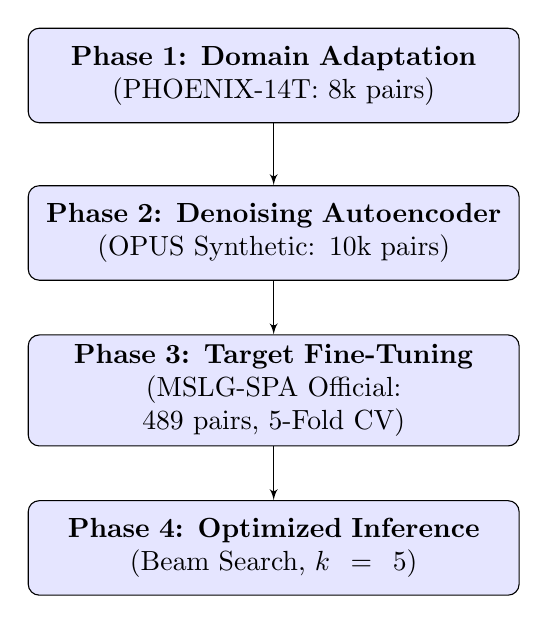
\begin{tikzpicture}[
    node distance=1.5cm,
    block/.style={rectangle, draw, fill=blue!10, text width=6cm, text centered, rounded corners, minimum height=1.2cm},
    line/.style={draw, -latex'}
]
    % Nodes
    \node [block] (phase1) {\textbf{Phase 1: Domain Adaptation}\\(PHOENIX-14T: 8k pairs)};
    \node [block, below of=phase1, node distance=2cm] (phase2) {\textbf{Phase 2: Denoising Autoencoder}\\(OPUS Synthetic: 10k pairs)};
    \node [block, below of=phase2, node distance=2cm] (phase3) {\textbf{Phase 3: Target Fine-Tuning}\\(MSLG-SPA Official: 489 pairs, 5-Fold CV)};
    \node [block, below of=phase3, node distance=2cm] (phase4) {\textbf{Phase 4: Optimized Inference}\\(Beam Search, $k=5$)};
    
    % Edges
    \path [line] (phase1) -- (phase2);
    \path [line] (phase2) -- (phase3);
    \path [line] (phase3) -- (phase4);
\end{tikzpicture}
\caption{The proposed four-phase transfer learning pipeline utilizing mBART-50.}
\label{fig:pipeline}
\end{figure}

\textbf{Phase 1: Domain Adaptation (PHOENIX-14T).} I hypothesized that sign languages, despite regional differences, share universal typological features regarding information density and grammatical omission. I conducted a structural warm-up by fine-tuning the base mBART-50 model on approximately 8,000 pairs from the German PHOENIX-2014-T dataset (translating DGS Glosses to German text).

\textbf{Phase 2: Denoising Autoencoder Training.} Using the 10,000 synthetically generated pseudo-gloss pairs, I trained the model to project lossy representations back into fluent Spanish. This phase exposed the model to the specific vocabulary of Mexican Spanish and the syntactic constraints of the shared task.

\textbf{Phase 3: Target Fine-Tuning.} The model was subsequently fine-tuned exclusively on the 489 official MSLG-SPA pairs provided by the organizers. To validate performance internally, I employed a 5-Fold Cross-Validation strategy.

\textbf{Phase 4: Optimized Inference.} Inference was executed using beam search decoding. A beam width of 5 (\texttt{num\_beams=5}) was selected to explore a wider hypothesis space while avoiding over-penalization of shorter sequences. Early stopping was enabled to prevent the generation of repetitive tokens.

\subsection{Hardware Constraints and Optimization}
Training a 600-million parameter model requires computational resources. Due to hardware constraints, direct fine-tuning was impossible without encountering Out-Of-Memory (OOM) errors. I implemented several optimization techniques to bypass these limitations:
\begin{itemize}
    \item \textbf{Mixed Precision (FP16):} I utilized 16-bit floating-point precision, effectively halving the memory footprint of the model activations and weights while accelerating computation on Tensor Cores.
    \item \textbf{Gradient Checkpointing:} Rather than storing all intermediate activations during the forward pass, I recomputed them dynamically during the backward pass.
    \item \textbf{Gradient Accumulation:} I restricted the physical batch size to 2 and accumulated gradients over 4 consecutive steps before executing the optimizer update, mathematically simulating an effective batch size of 8.
\end{itemize}

\section{Results and Theoretical Limitations}

\subsection{Official Evaluation Results}
My system's performance was evaluated against the official blind test set provided by the organizers. For Subtask A (MSLG2SPA), my system achieved an official COMET score of 0.6813, alongside a BLEU score \cite{papineni2002bleu} of 16.6254 and a chrF score \cite{popovic2015chrf} of 45.7760. The overall Task Score was -0.5103. For Subtask B (SPA2MSLG), the system achieved an overall Task Score of -0.0644, alongside a BLEU score of 11.7564, a METEOR score \cite{banerjee2005meteor} of 0.3751, and a chrF score of 53.4845.

The COMET (Crosslingual Optimized Metric for Evaluation of Translation) metric \cite{rei2020comet} leverages pre-trained neural models to predict human judgments of translation quality, focusing on semantic equivalence rather than exact n-gram overlap. An official score of 0.6813 indicates a strong degree of semantic preservation and fluency, suggesting that the model successfully leveraged the synthetic pre-training phase to reconstruct grammatically correct Spanish from the sparse glosses.

\subsection{The Overfitting Paradigm}
Despite the positive semantic metrics (COMET), my methodological approach revealed severe theoretical limitations inherent in standard full fine-tuning. Updating all 600 million parameters of mBART-50 on a dataset of only 489 pairs is highly inefficient and prone to instability. 

This imbalance between parameter count and dataset size leads to two phenomena:
\begin{enumerate}
    \item \textbf{Pre-trained Knowledge Loss:} The large gradients generated by the small, highly specific target dataset aggressively overwrite the multilingual knowledge acquired during pre-training, causing the model to lose its foundational understanding of Spanish syntax.
    \item \textbf{Overfitting:} The model rapidly memorizes the specific vocabulary and exact phrasing of the 489 training pairs. Consequently, it loses the ability to generalize to unseen test instances or natural variations in MSL glossing.
\end{enumerate}

My observations during Phase 3 training confirmed rapid validation loss degradation after only a few epochs. Standard full fine-tuning simply lacks the necessary regularization mechanisms to map a highly divergent grammar (MSLG) into a high-resource language space (Spanish) when bounded by extreme data scarcity. This explains why the n-gram overlap metrics (like BLEU) remained average, even while the semantic intent (COMET) was reasonably preserved.

\section{Reproducibility}
To adhere to open science standards and ensure the reproducibility of these results, the source code, including the rule-based augmentation script (\texttt{glosado.py}) and the training notebooks, has been made publicly available via GitHub: \url{https://github.com/mikebeth/MSLG-SPA-2026}. 

Furthermore, the foundational models and datasets utilized in my pipeline are publicly accessible: the base \texttt{mBART-50 Large} architecture can be acquired via the HuggingFace Model Hub, the synthetic data was derived from the OPUS corpus \cite{tiedemann2012parallel}, and the domain adaptation was conducted using the open-source PHOENIX-2014-T dataset \cite{camgoz2018neural}.

\section{Conclusion and Future Work: The Case for LoRA}

In this paper, I presented a pipeline for bidirectional translation between Mexican Sign Language glosses and Spanish, leveraging the mBART-50 architecture and synthetic data augmentation. While my system established a baseline performance highlighted by a highly competitive COMET score of 0.6813---which proves the model's capacity to preserve core semantic meaning---the core limitation lies in the parameter update strategy under data scarcity.

Future iterations of SLT systems operating in low-resource environments must abandon full fine-tuning in favor of Parameter-Efficient Fine-Tuning (PEFT) methodologies. Specifically, the integration of \textbf{Low-Rank Adaptation (LoRA)} \cite{hu2021lora} represents a viable path forward. LoRA operates by freezing the pre-trained model weights and injecting trainable rank decomposition matrices into the Transformer's self-attention layers. 

By drastically reducing the number of trainable parameters, LoRA regularizes the training process. This would allow the model to learn the unique morphological mapping between MSL and Spanish without destabilizing the foundational linguistic representations embedded within mBART-50, ultimately resolving the overfitting paradigm and enabling improved structural generalization in future MSLG-SPA translation efforts.

\section*{Declaration on Generative AI}
Generative AI services such as Chat DeepSeek were employed to refactor, optimize, and improve the codebase. Following the use of these services, all generated content was reviewed and edited as necessary. Full responsibility for the publication's content is assumed.

\bibliography{references}

\end{document}
